\chapter{Background}
\label{chap:background}
Image classification refers to a task that requires from method to determine the categories to which picture belongs. Such challenges that utilize standard datasets like ImageNet and PASCAL VOC limit this problem to a question if objects of particular classes presented on the image \cite{Russakovsky2015ImageNet, Everingham2010PASCAL-VOC}. However, real-world settings might require extending this question to more general one \cite{Wang2016CNN-RNN:Classification}. For instance, in this study, the search extended beyond merely objects to include other image properties including color, weather, action, and sceneries. %In other words, image classification system should be able to find a correct placement of a picture in a multi-dimensional space of categories.

% \section{Image classification}
% definition of image classification

\section{Deep convolutional neural networks}

A standard neural network consists of computational units called neurons. Neurons are connected to each other in particular way to form a network. Neurons in such networks are organized in groups or ``layers'' for computational efficiency reasons since it allows to apply vector operations \cite{cs231n-nn1}.  Each input connection to a neuron has dedicated weight. Non-liner \textit{activation function} use these input weights to determine when to activate particular neuron and send a signal further \cite{Schmidhuber2015DeepOverview}. Activation function can be different, however recent years ReLU function is mostly used in modern DNN due to its computational efficiency and good output results \cite{relu, Krizhevsky2012ImageNetDNN}. The ``depth'' of the neural network is identified as an amount of layers except input one \cite{Schmidhuber2015DeepOverview}.

The process of \textit{training} the neural network is optimization of each neuron input weights in such way that the particular input to a network will produce desired output. This optimization is achieved by first introducing loss function which represents how ``far'' given output is from the desired one. After that, on each iteration of training, by calculating gradients of a loss function on given weights, the system determines how it should adjust weights to decrease the computed loss \cite{cs231n-opt1}. Modern DNNs use backpropagation approach of gradient calculation due to its efficiency \cite{cs231n-opt2}. 

Convolutional Neural Networks (CNN) have the same core ideas as any other neural networks except that CNN architectures assume that the inputs are images \cite{cs231n-conv}. Unlike conventional neural networks, instead of processing images pixel-by-pixel CNN is searching for patterns in image patches of different sizes. Each convolution can also be perceived as a feature extractor, such as the one that detects particular edge angle or color. Such convolution functions are also organized in layers where output features from one layer is an input data for next convolutional filters. Therefore, an end system consists of filters cascade, where, similar to human vision, low-level features, like edges, are recognized on the fist levels, and higher levels trigger on more complex features like different shapes and patterns \cite{Zeiler2014VisualizingNets}

The main difference between machine learning approach and deep convolutional neural networks is that the former one has an additional step of supervised feature extraction. In contrast, in deep learning approach feature extraction happens automatically by the internal network itself. Therefore DNN can be considered as a ``black box'' system. For instance, in the case of image classification, such system will have raw picture pixels as an input and classified category numbers as output.

To improve the generalizability of results and to be able to compare networks with different hyperparameters the common approach is to use dataset splitting where an image collection is partitioned into three parts \cite{cs231n-cls}. The first part is employed directly for training, while the second part, called \textit{validation set}, is used to compare different architectures and control overfitting.  Overfitting is a state of the system when it optimizes to a noise in a training data instead of searching the underlying patterns \cite{cs231n-nn1}. Such optimization can potentially reduce the generalizability of the system and should be avoided \cite{cs231n-nn1}. The usual way to control overfitting of the model is to check system performance on a validation set periodically \cite{cs231n-nn3} during the training process. If the loss computed on a training set gets smaller with more iterations, but validation loss increases, then it is a sign that the model is starting to overfit on the training set \cite{cs231n-nn3}. Therefore, to be able to monitor the generalizability of the method validation set should not contain any images from the training set. The third part of the dataset, which is called \textit{test set}, is used for a final evaluation of the method. The separation between validation and test sets is important for the similar reason as with separation between training and validation sets. When different network implementations are compared using validation set, and the best one is selected, hyperparameters can overfit on the validation set similar to the process network overfitting on the training set \cite{cs231n-cls}. Meaning that chosen parameters will be optimized for the particular images in the validation set. Therefore, it is important to test the final system on a separate set of pictures, which CNN has not seen at any time during the training process. According to Andrew Ng, The common ratio between these tree sets is 60\%/20\%/20\%, where the training set gets 60\% of images while validation and test sets receive 20\% each \cite{Ng2016NutsLearning}.
% train, val, test split
% different layers
% overfitting
% backpropagation

\section{Multi-label image classification}
Opposite to a single-label image classification, in multi-label case picture can belong to more than one category. Several labels can both describe all objects presented on the picture and characterize the objects or picture itself.

There are two group of multi-label image classification methods:
\begin{itemize}
    \item That process parts of the images and use CNN to find a single label for each of the part \cite{Wei2016HCP, Yang2015, Ren2016}.
    \item That train CNN on the whole picture, similarly to single label methods, but use different loss functions that take several labels into account \cite{Gong2013DeepRanking},
\end{itemize}

An example of the first type of network is described by Wei et al. in their paper ``HCP: A Flexible CNN Framework for Multi-Label Image Classification''  \cite{Wei2016HCP}. The core idea of the proposed method is to reuse already developed CNNs that were trained to classify single-labeled pictures in a multi-label scenario. The authors proposed deep CNN infrastructure called ``Hypotheses-CNN-Pooling'' (HCP) to achieve this. Its architecture is shown on Figure \ref{fig:hcp-net}.

\begin{figure}[h!]
    \centering
    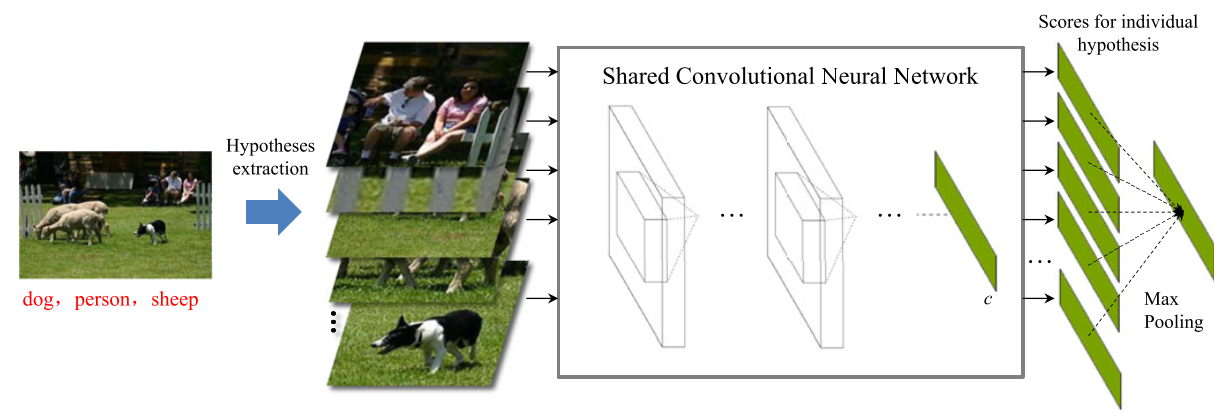
\includegraphics[width=\textwidth]{hcp-net}
    \caption{Hypotheses-CNN-Pooling infrastructure \cite{Wei2016HCP}}
    \label{fig:hcp-net}
\end{figure}

The whole classification pipeline consists of the following steps:
\begin{enumerate}
    \item Applying state of the art object detection technique (for example BING \cite{Cheng2014} or EdgeBoxes \cite{Zitnick2014}) to get the set of hypothesis,
    \item Using proposed hypothesis selection method reduce the number of initial hypotheses,
    \item Use pre-trained CNN to assign single label for each hypothesis,
    \item Use cross-hypothesis max-pooling to create the vector of labels found on the whole picture.
\end{enumerate}

Authors claim of getting up to 90.9\% of Mean Average Precision (which is defined in PASCAL Challenge \cite{Everingham2010PASCAL-VOC}) on PASCAL VOC 2012 image dataset.

Yang et al. proposed similar infrastructure, but extended it with additional large-margin nearest neighbor (LMNN) CNN that incorporates knowledge of ground truth bounding boxes of the training set to improve results  \cite{Yang2015}. This extra layer tries to find similar objects in the test image to the ones extracted from the training set (ground-truth object set) independently from the other layer that employs more usual CNN. Results from the both layers are taken into account in the final prediction vector.

The method described by Girshik et al. in ``Rich feature hierarchies for accurate object detection and semantic segmentation'' paper also highly rely on the ground-truth bounding box during the training phase \cite{Girshick2014}. In particular, generated hypothesis are ranged based on the overlap with ground-truth box.

Oquab et al. proposed method that also use bounding box information to produce labels for training images \cite{Oquab2014TransferringMidLevel}. Specifically, they propose to generate around 500 square patches from the picture and put a single label on each patch dependently on the overlap with the ground truth bounding box. Patches which intersect with two or more objects are filtered out, and the once which do not intersect with any objects are labeled as a background. Example training data generated from the image and ground-truth information is shown on figure \ref{fig:patches-example}.

\begin{figure}
    \centering
    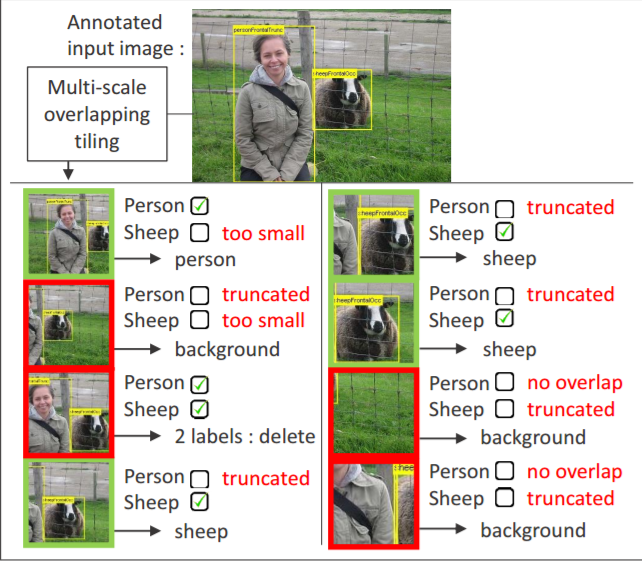
\includegraphics[scale=0.35]{patches-example}
    \caption{Training data generation example using patching method \cite{Oquab2014TransferringMidLevel}}
    \label{fig:patches-example}
\end{figure}

Currently, the first type of multi-label classification methods with image partitioning show improved performance compared to the ones that use the whole pictures \cite{Wei2016HCP, Yang2015, Ren2016}. However, such methods require having either ground truth bounding box encoded in metadata in addition to labels which identifies the location of all objects on the image \cite{Chen2015ContextualizingClassification, Dong2013Subcategory-AwareClassification}, or pre-trained single-label classifier for the same set of categories \cite{Wei2016HCP}. In addition, this approach might be more suitable for searching for objects in the picture, but not perform as good to assign labels describing the whole image since it processes only part of a picture at a time. For instance, the dataset used in this study had label \textit{alone} that separates images with single objects, or \textit{landscapes} which characterize the whole picture. These kinds of categories might be challenging to classify using method that splits an image.

In contrast to previous papers, Gong et al. applied CNN to the whole picture without partitioning \cite{Gong2013DeepRanking}. The main contribution of this study was not to produce new multi-label classification method, but to compare different loss functions in multi-label classification context. Results showed that weighted approximated-ranking loss (WARP) improved the classification performance of the categories with a small number of pictures which can be an essential factor for unbalanced datasets.

Wang et al. in their research were also trying to improve multi-label image classification performance for realistic image collections \cite{Wang2016CNN-RNN:Classification}. Authors point out a problem with methods that transforming multi-label task into a single-label one. Researchers identify the lack of modeling semantic dependencies between categories in such methods. The main reason for this is that such approaches treat image categories completely independently, while some of the labels might occur together more often than others. To solve this problem, the authors propose to utilize Recurrent Neural Network (RNN) in addition to CNN, which can model semantic relevance between images.

Most of the presented methods use so-called transfer learning technique in different ways to improve their results and to utilize the work from the other studies to their benefit. Brief description and motivation behind this approach presented in next section.

% \section{Caffe framework}

% pipeline of computations going through layers
% sigmoid cross entropy

\section{Transfer learning}
\label{sec:transfer-learning}

Usually, the usage of deep learning approach adds additional requirements: to have enough processing power and big enough image dataset. One of the most common methods to reduce these constraints called \textit{transfer learning}. The main principal behind it is to reuse ``knowledge'' of a pre-trained neural network on one task and transfer this knowledge to another one \cite{Pan2010TransferLearningSurvey, Oquab2014TransferringMidLevel}. This idea appeared when people noticed that first layers of most CNNs learn to trigger on the same features like corners, edges, color conjunctions, therefore there is no need to discover them in each network \cite{Zeiler2014VisualizingNets}.

There are two types of transfer learning \cite{Yosinski2014HowTransferable}:
\begin{itemize}
    \item With frozen layers, when layers copied from the pre-trained network do not change their weights during the backpropagation phase, in other words, their learning rates are set to zero,
    \item Fine-tuning, when copied layers only start with pre-trained weights, but during the training phase adjust just their values like all other layers.
\end{itemize}

Oquab et al. describe in detail the usage of transfer learning for multi-label classification. In particular, they show how pre-trained network on one category set can be used to find labels for more general categories (for example source categories might include different dog breeds while target set may contain only general label ``dog'') or even entirely new ones \cite{Oquab2014TransferringMidLevel}. Insights provided in this research will be applied in the project since target NTB dataset also has a different set of categories compared to the ones available in the standard image collections.

The transfer learning method employed in this project, which is described in the next chapter, allowed to ease dataset size and performance requirements needed for successful system training. Recent studies also suggest that the usage of a pre-trained model can improve the generalizability of the final image classification system in contrast to the system trained on the target dataset from scratch \cite{Yosinski2014HowTransferable, Oquab2014TransferringMidLevel}.

\section{Real-world datasets}
Some datasets like PASCAL VOC or NUS WIDE are created from realistic pictures that contain several objects or people in different combination and interactions between them \cite{Everingham2010PASCAL-VOC, Chua2009NUS-WIDE}. Creators of such datasets, as well as other researchers, argue that real-world images are more likely to have multi-label nature by having both multiple entities in the picture as well as such category set that can describe image or object in several prospectives \cite{Wang2016CNN-RNN:Classification, Dong2013Subcategory-AwareClassification, Everingham2010PASCAL-VOC, Chua2009NUS-WIDE}. Wang et al. poit out that in addition to objects, such images can contain parts of some entities, scenes, and actions \cite{Wang2016CNN-RNN:Classification}. Authors also identify the challenge of small objects on such images that can be ignored by classification methods, especially when full pictures are processed in a neural network.

Except for the picture collection itself, dataset should also contain metadata for image and a defined set of categories. While datasets described earlier consist of realistic pictures, the set of categories and therefore images were designed and moderated for the purpose of further training and comparison of image classification systems. Therefore, there is still a question on how different state of the art methods can be applied to datasets that were created for other reasons and how their metadata usage can be maximized. In addition to realistic pictures, such datasets can have additional challenges connected with a unique set of labels, a less balanced size of categories, a big number of both systematic and random errors.

\subsection{Current state of the NTB dataset}
As it was mentioned earlier, NTB provided their labeled image collection for the purpose of these project. Currently, NTB dataset contains around one million of manually annotated pictures and more than ten millions of images without labels. Therefore, the fist usage of the automatic image classification system for the company is to propagate annotations on other images from the collection. NTB has its unique set of categories organized in a tree structure. The company uses these tags to provide a solution for pictures search to their customers. Therefore the second application of the system would be to incorporate an image classification in this search solution. More in-depth analysis of the NTB dataset will be presented in Section \ref{sec:dataset-analysis}.

% own set of categories, have to trafsfer them as many as possible